\section{Experiments}
Our experiments aim to answer the following questions:
\begin{enumerate}
    \item How does our proposed Prioritized Replay Buffer compare against existing baseline approaches? (See Section~\ref{sec:comp_baselin})
    \item Does the performance of our proposed Prioritized Replay Buffer follow the theoretical analysis in Section~\ref{sec:sum_tree} in terms of the fanout size $K$? (See Section~\ref{sec:perf_prioritized})
    \item How does our proposed locking mechanisms for the prioritized replay buffer reduce the synchronization overhead compared with using a global lock? (See Section~\ref{sec:perf_prioritized})
    \item What is the performance improvement when plugging in our prioritized replay buffer implementation into existing RL frameworks? (See Section~\ref{sec:comp_existing})
\end{enumerate}

\subsection{Experimental Setup}
We conduct our experiments on 56-core Intel(R) Xeon(R) Gold 5120 CPUs with 128GB DDR4 memory and a Nvidia TITAN Xp GPU with 12GB GDDR6 memory as the accelerator. We implement the synchronization mechanism using pthreads \cite{pthread} and the training of neural networks using LibTorch \cite{pytorch}. We test our framework on reinforcement learning algorithms including DQN \cite{dqn} and DDPG \cite{ddpg}. DQN targets at discrete action space while DDPG and SAC targets at continuous action space. We use \textit{LunarLander-v2} \cite{openai_gym} environment to test the algorithms. In all our experiments, the desired ratio between the throughput of the data collection and the data learning (update\_interval) is set to 1.

\subsection{Baseline Approach}
In this work, we use RLlib \cite{ray_rllib} as our baseline. RLlib is an open source implementation of parallel and distributed framework for training reinforcement learning agents written in Python \cite{python}. For fair comparison, we use the same amount of cores when running the experiments. We also compare with the Prioritized Replay Buffer implementation in open source RL framework tianshou \cite{tianshou}.

\subsection{Comparison with Baseline Approaches}\label{sec:comp_baselin}
\begin{figure}
    \centering
    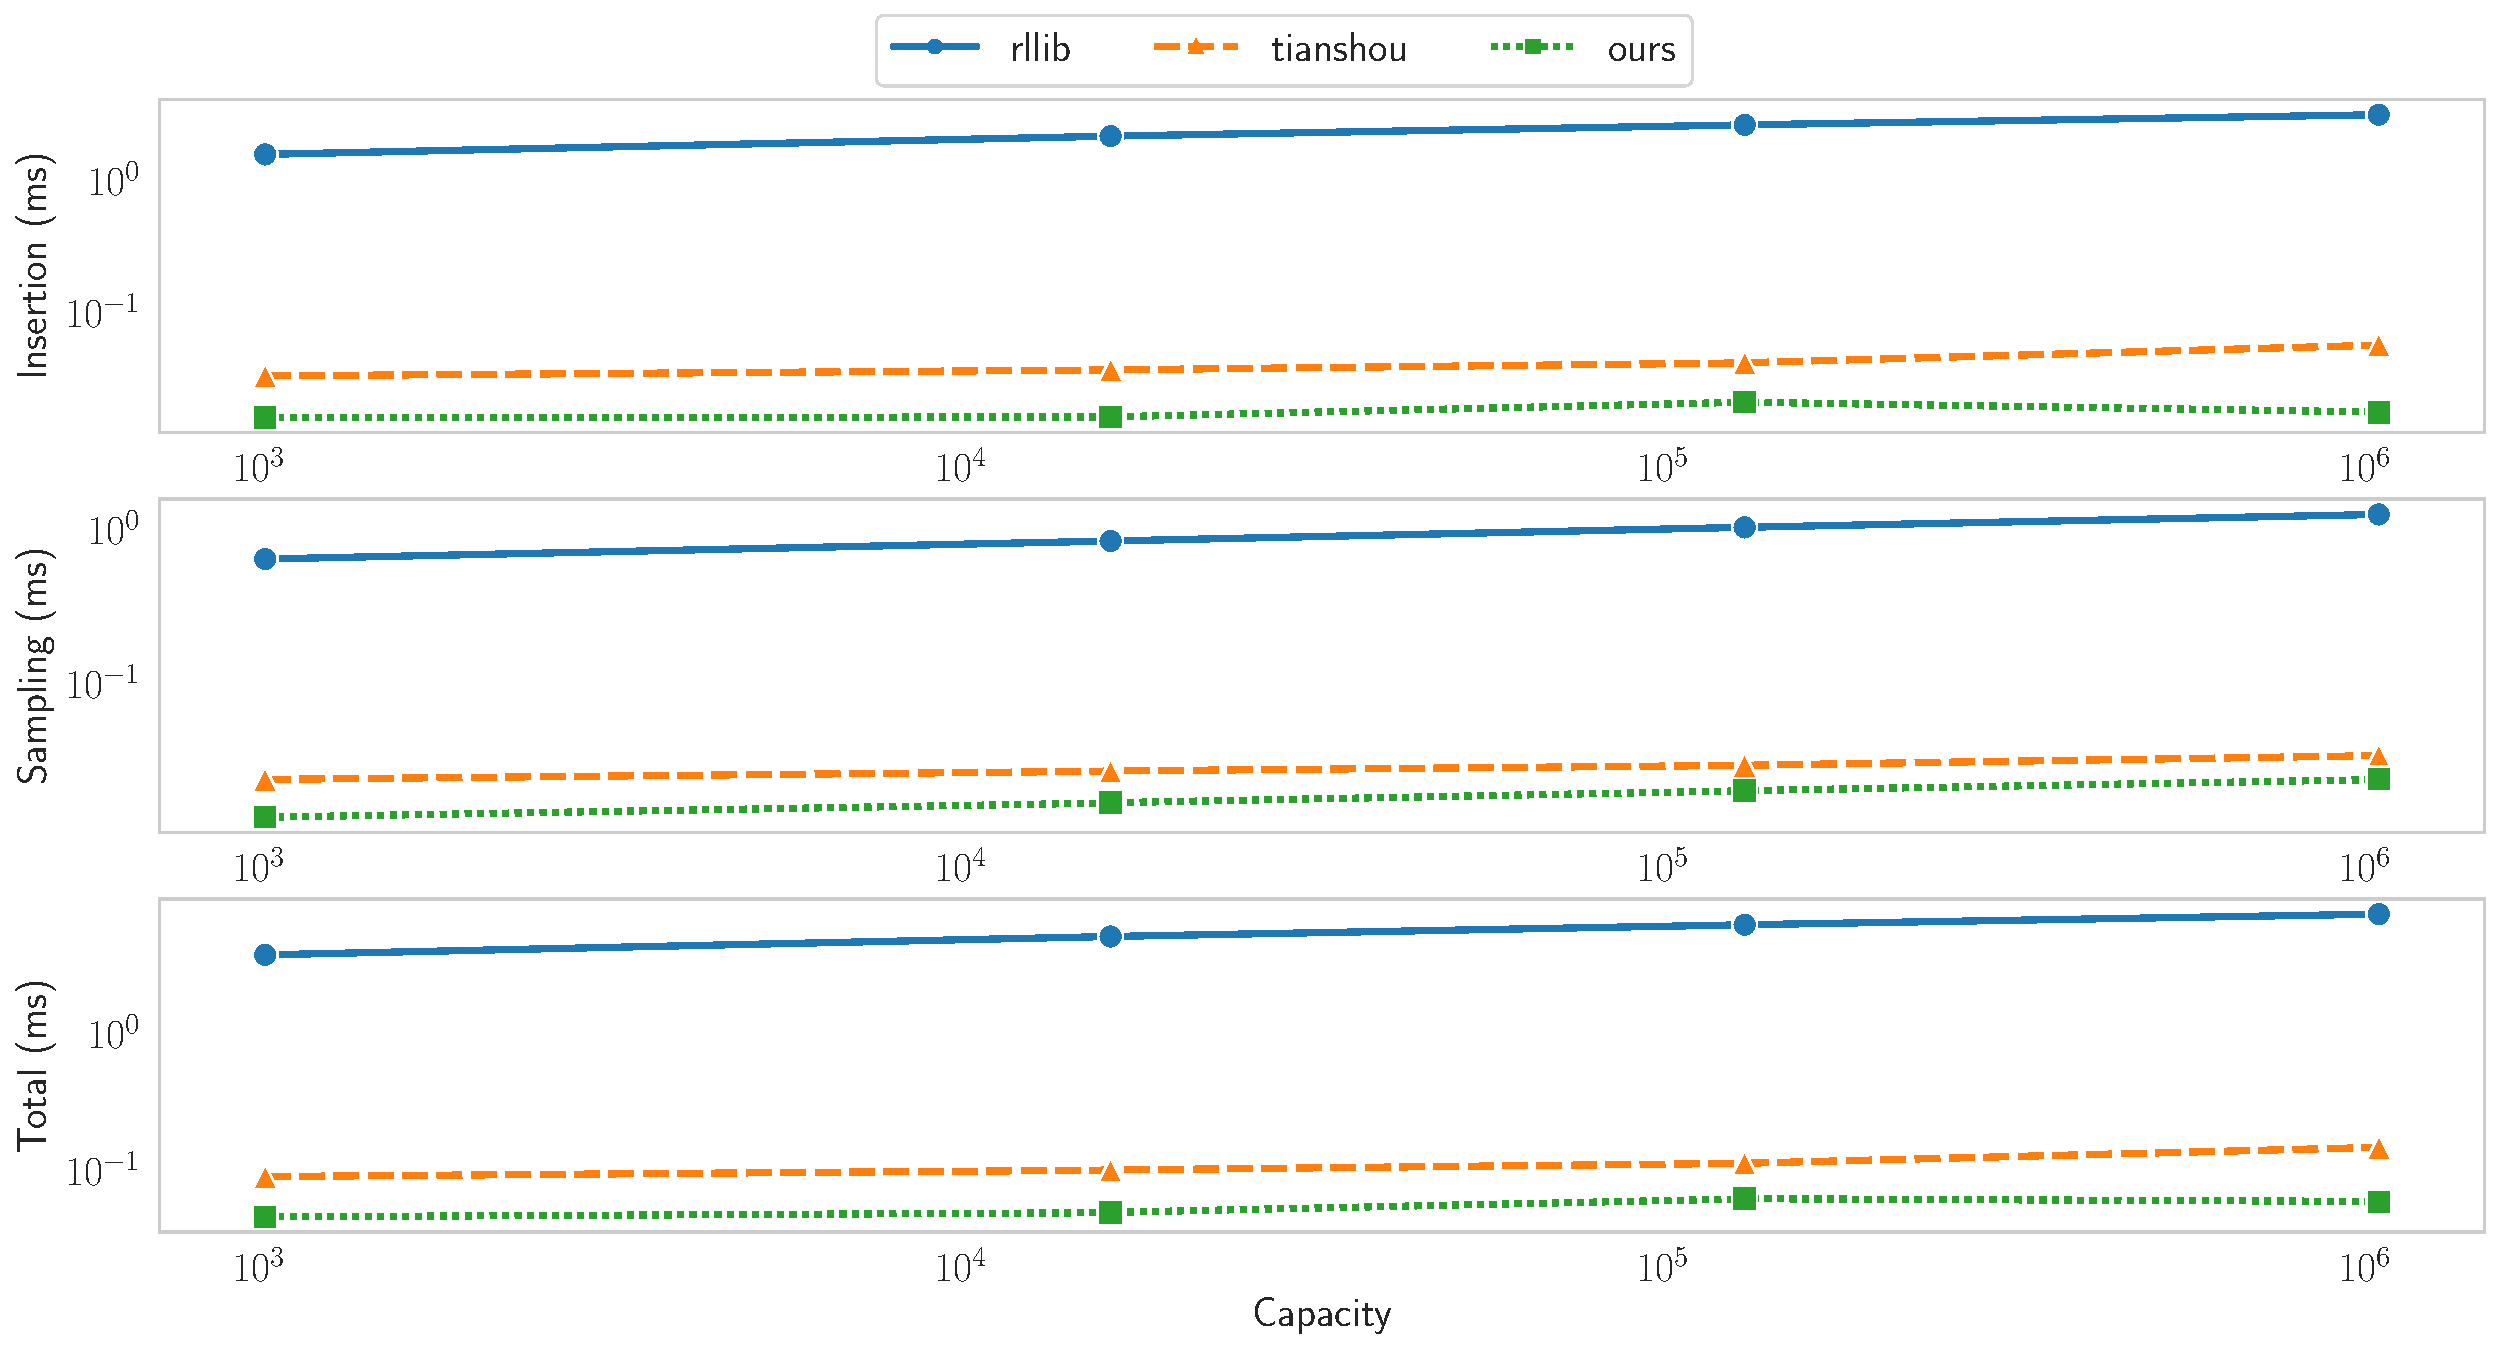
\includegraphics[width=\linewidth]{sum_tree_comp.pdf}
    \caption{Comparison with the baseline approach}
    \label{fig:baseline_comp}
\end{figure}

We show the latency of insertion and sampling of the Replay Buffer with various sizes in Figure~\ref{fig:baseline_comp}. We compare our $K$-ary sum tree based implementation with RLlib \cite{ray_rllib} and tianshou \cite{tianshou}. Overall, our approach reduces the total latency by around 4x compared with tianshou \cite{tianshou} and around 100x compared with RLlib \cite{ray_rllib}. Note that the latency of the Prioritized Replay Buffer operations in  RLlib increases in linear while the latency of our implementation increases in sub-linear. This suggests our $K$-ary based Prioritized Replay Buffer has better scalability compared with \cite{ray_rllib}.

\subsection{Performance of the Prioritized Replay Buffer}\label{sec:perf_prioritized}
\begin{figure}
    \centering
    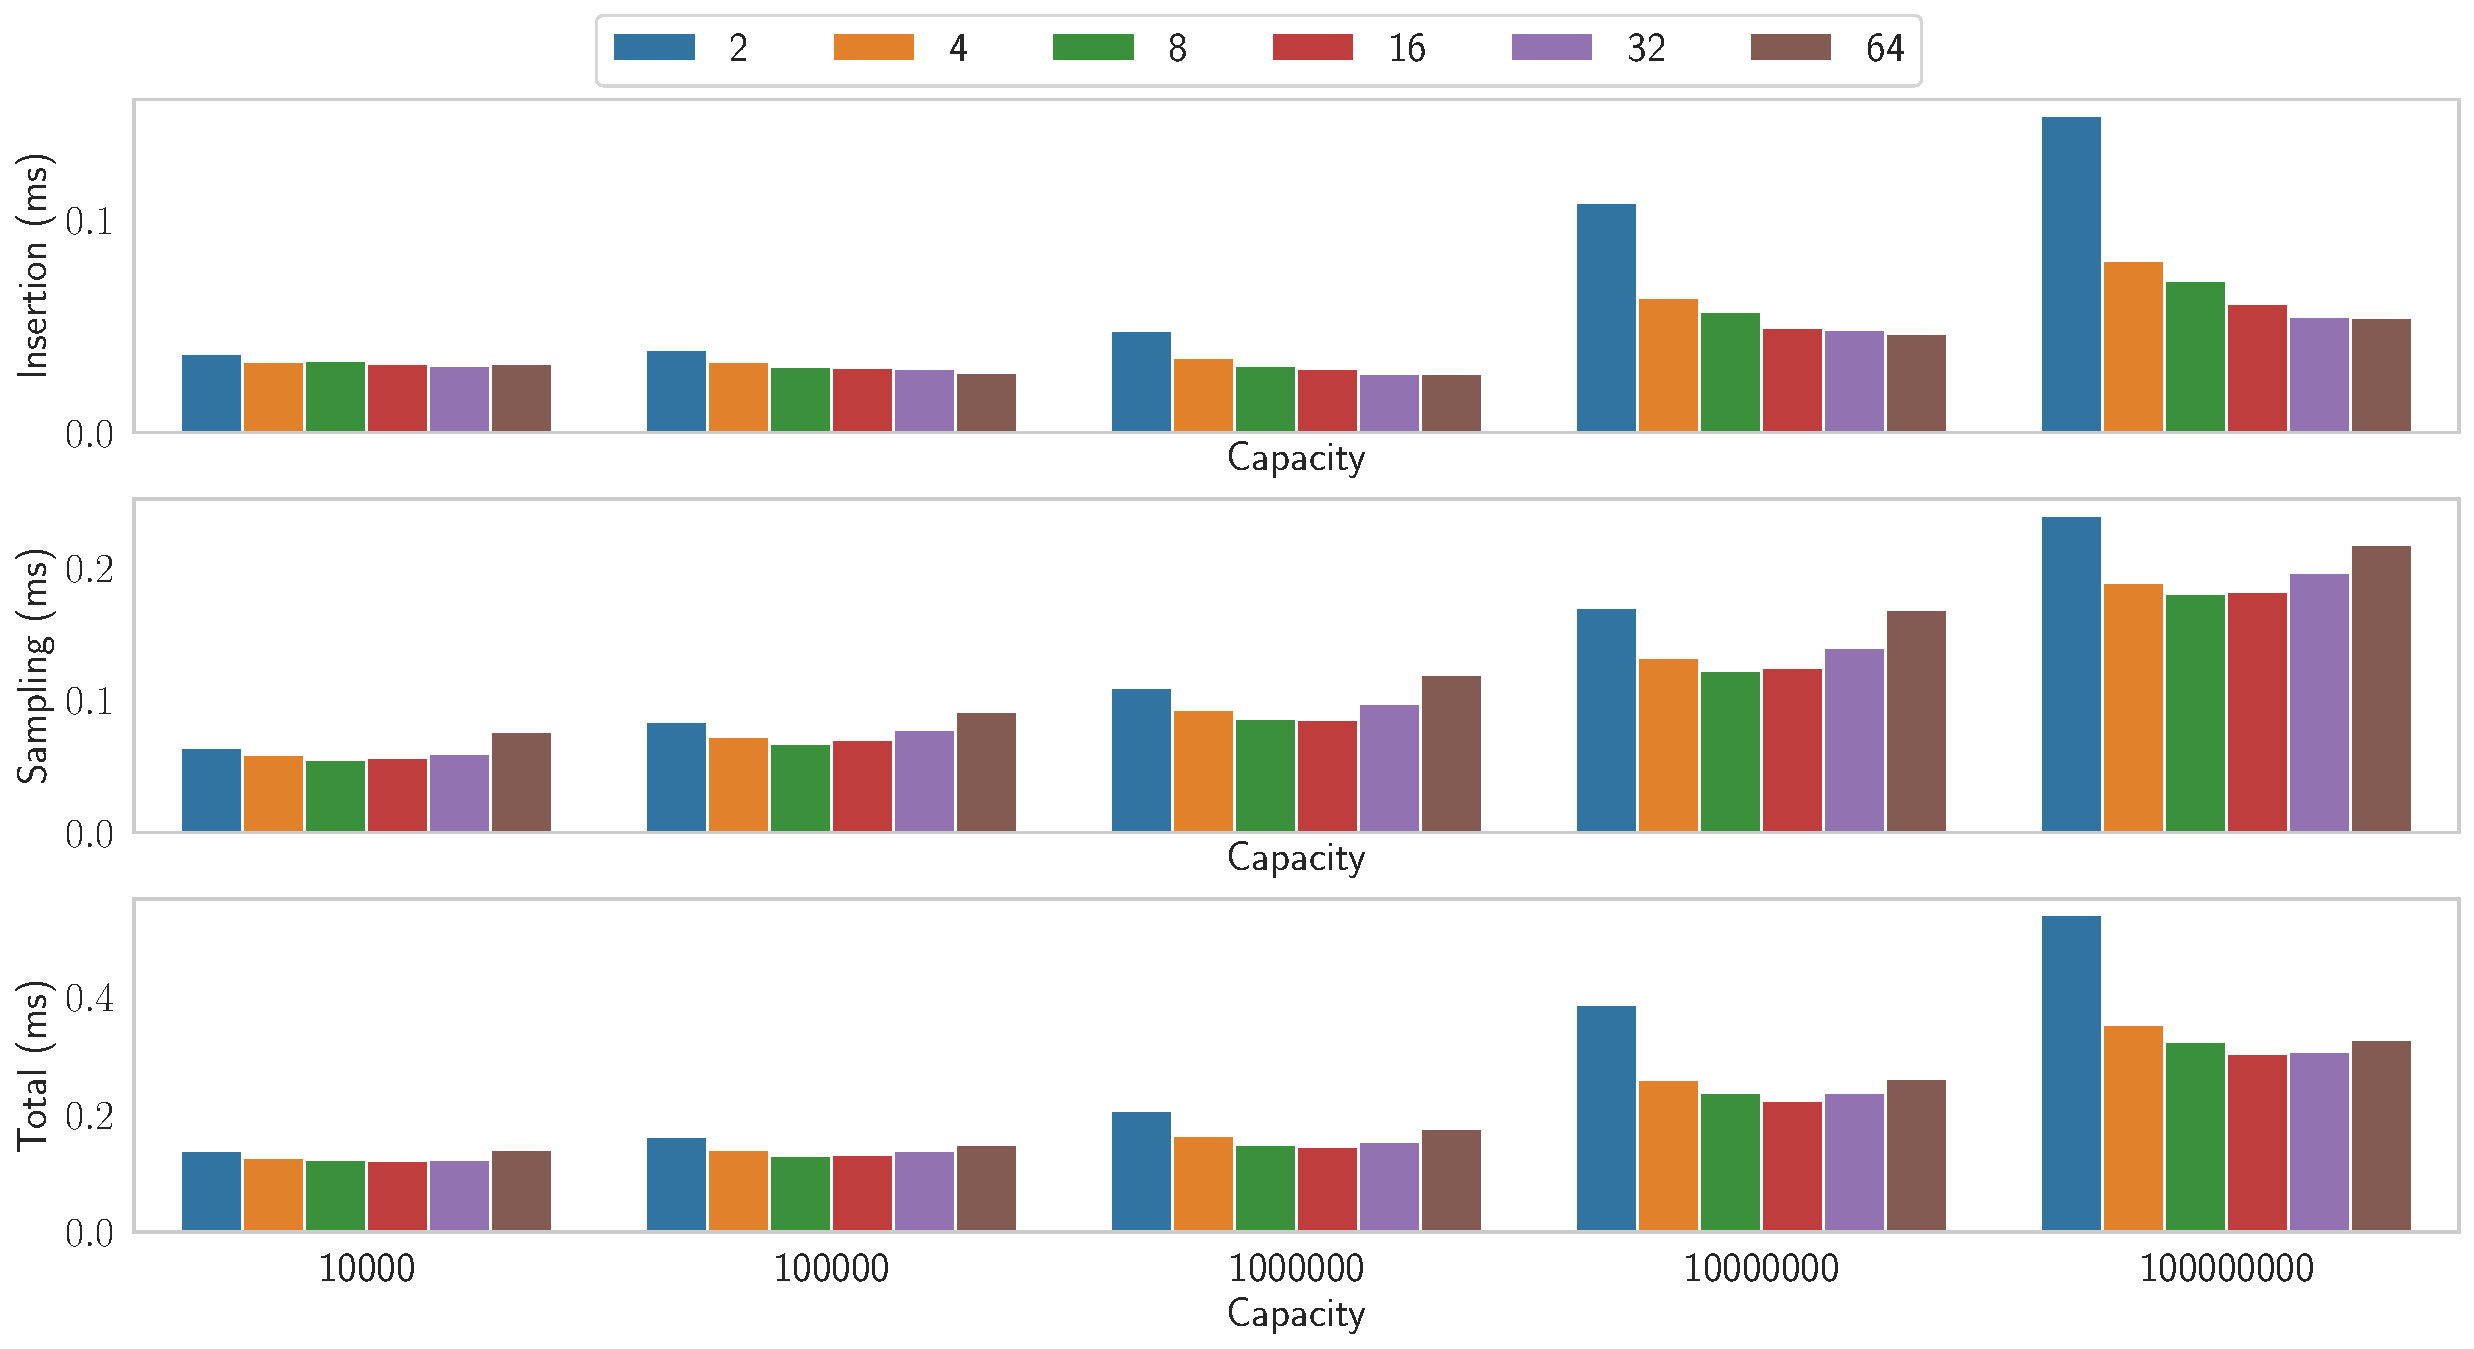
\includegraphics[width=\linewidth]{sum_tree_ops.pdf}
    \caption{Latency of various Prioritized Replay Buffer operations with various fannout $K$}
    \label{fig:k_ary_sum_tree}
\end{figure}
\subsubsection{Effect of fanout $K$}
In order to answer question 2, we show the latency of insertion and sampling of various $K$ in Figure~\ref{fig:k_ary_sum_tree}. We also vary the capacity of the Replay Buffer to demonstrate the scalability. First, we observe that the latency of insertion decreases when $K$ increases. This matches our theoretical performance analysis because the latency is proportion to the height of the tree. The height of the tree decreases when $K$ increases. Second, we observe that the latency of sampling first decreases to a local minimum and then increases as $K$ increases. This also matches with our theoretical analysis because as $K$ increases, the latency increase of search over each level starts to dominate the latency decrease with fewer number of levels. In order to choose the optimal $K$, we simply perform profiling of insertion and sampling to obtain the total latency. In our experimental machine, $K=16$ yields the best result.

\subsubsection{Effect of synchronization optimization}

\begin{figure}
    \centering
    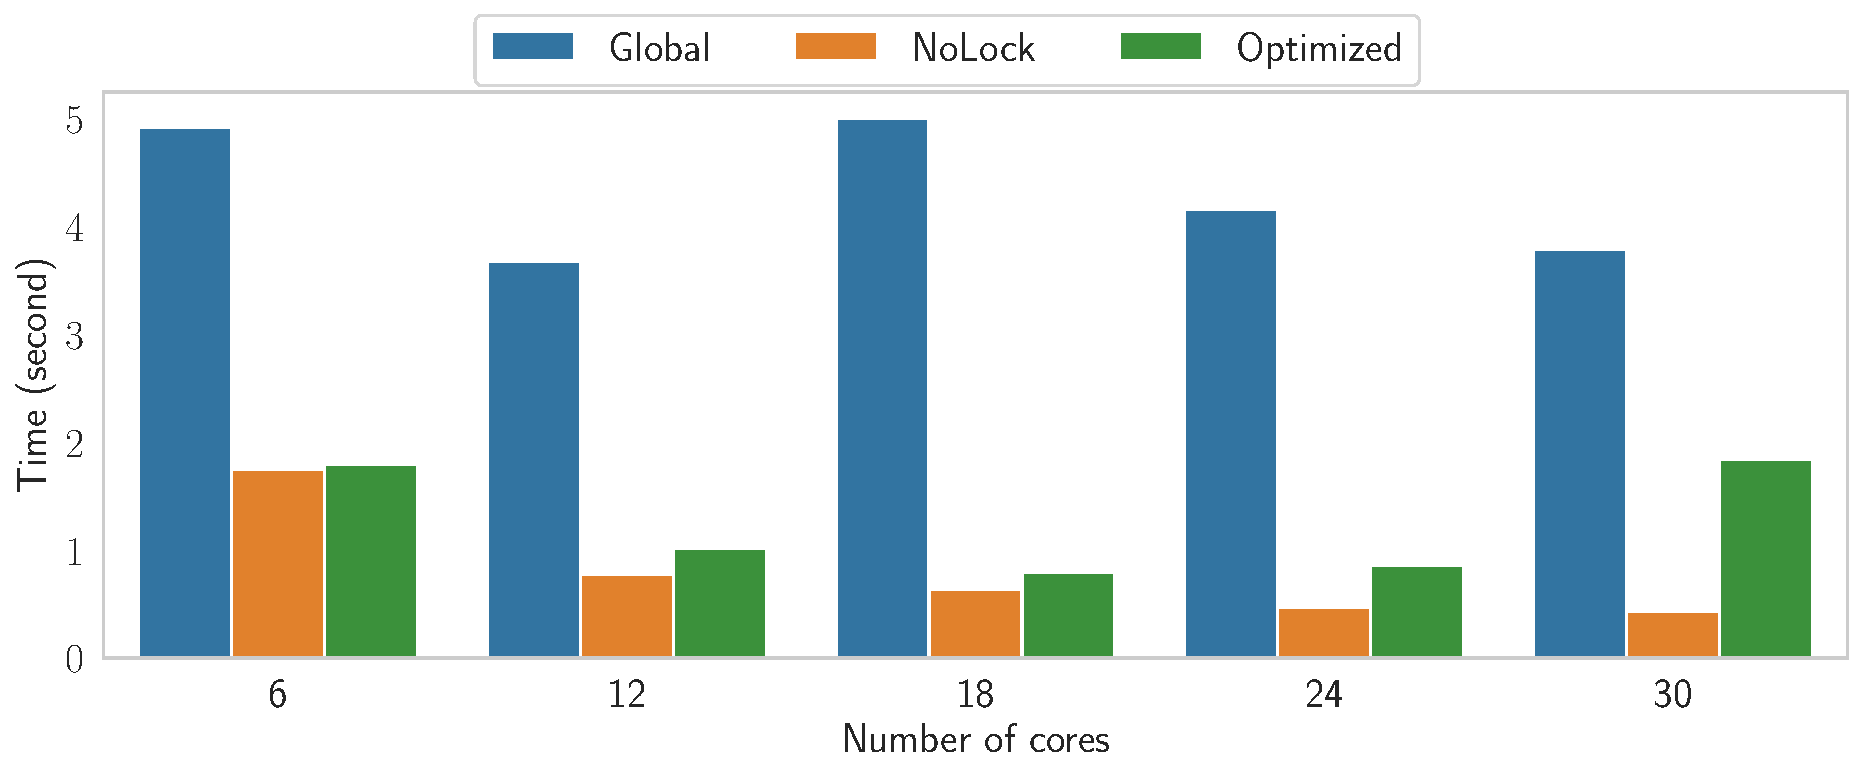
\includegraphics[width=\linewidth]{sum_tree_sync.pdf}
    \caption{Execution time of the Prioritized Replay Buffer with various synchronization methods}
    \label{fig:scalability}
\end{figure}
In order to answer question 3, we show the execution time of 5000 iterations versus the number of CPU cores using a global lock, no lock and our proposed synchronization optimization in Section~\ref{sec:thread_safe_prb}. Although the results of computations without using lock are wrong, it provides an upper bound on the performance. We observe that our proposed thread-level synchronization enables 1.01x$\sim$5x increase of the execution time compared with the minimum achievable execution time; and achieves 2x$\sim$5x improvement against using a global lock. Moreover, our design scales well in the number of CPU cores.


% In order to answer question 2 and 3, we compare the throughput speedup of our proposed prioritized replay buffer using $K$-ary sum tree with the implementation using a binary sum tree with a single global lock. To do so, we spawn 4 threads, each thread runs sampling and priority update on the shared replay buffer using random data 1000 times. The throughput speedup is shown in Figure~\ref{fig:k_ary_sum_tree}. First, we notice that all the throughput speedup is above 4. This is because using a global lock on the replay buffer limits the maximum number of running thread to 1. On the contrary, our proposed locking mechanism provides linear scalability.

% To answer question 3, we observe that there exists a local maximum of the throughput speedup when increasing the fanout size of the sum tree $K$. For example, we choose $K=256$ when the size of the replay buffer is $1000$, $K=128$ when the size of the replay buffer is $10000$ and $K=64$ when the size of the replay buffer is $100000$. It is also worth noticing that the optimal $K$ decreases as the size of the replay buffer increases. This is because as the size of the replay buffer increases, the linear search of the child nodes in one level dominates.

% \subsection{Scalability Analysis}\label{sec:scale_analysis}
% We compare our proposed parallel framework with various CPU cores against the sequential version on various RL algorithms. We show the scalability of our propose framework in Figure~\ref{fig:scalability}. We notice that the performance scales in linear when the number of CPU cores is below 4. The scalability saturates when the number of cores is above 6. The reason is that the bottleneck of the system becomes the GPU, which performs gradient computations and aggregations.





\subsection{Performance improvement of existing frameworks using our proposed replay buffer}\label{sec:comp_existing}
In order to show the superiority of our proposed Prioritized Replay Buffer, we write a Python binding of the C++ implementation and plug it into existing open source RL framework RLlib \cite{ray_rllib}. We show the latency of each training step of two RL algorithms in Figure~\ref{fig:library_perf}. 
Overall, we achieve 1.19x$\sim$ 1.75x performance improvement using various CPU cores.
The speedup decreases as the number of CPU cores increases. This is because the proportion of the replay buffer operations time decreases for each core and the bottleneck shifts to training the neural networks.

\begin{figure}
    \centering
    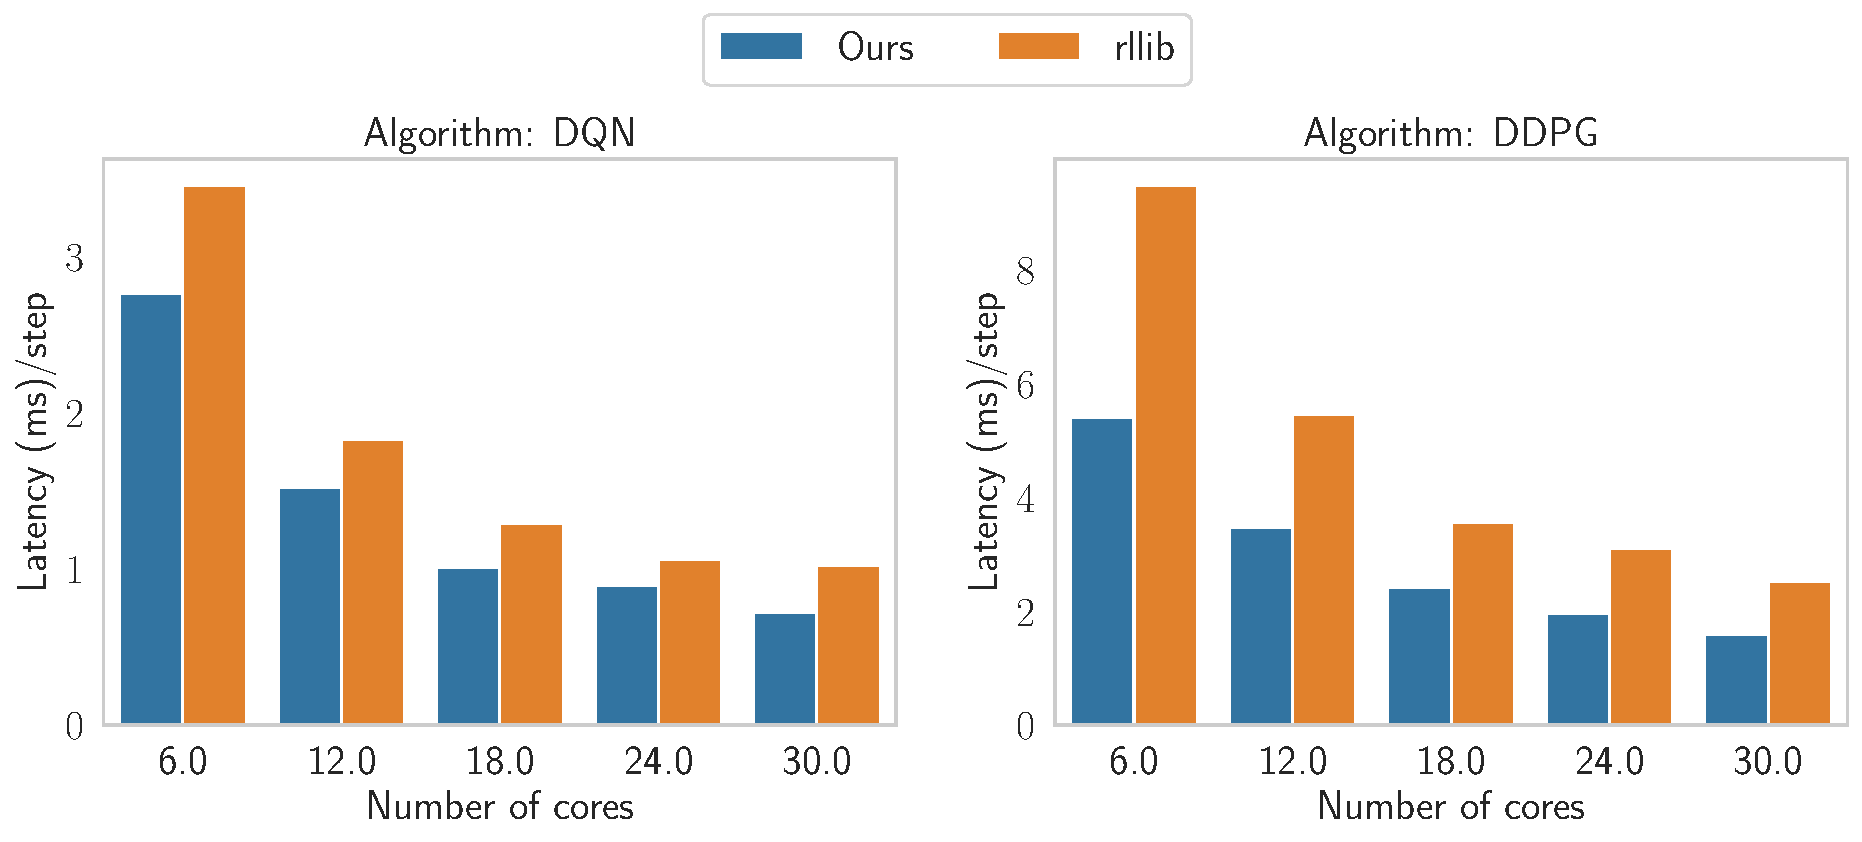
\includegraphics[width=\linewidth]{state_of_the_art.pdf}
    \caption{Overall speedup by plugging our prioritized replay buffer implementation into existing open source reinforcement learning libraries.}
    \label{fig:library_perf}
\end{figure}

% \subsection{The agent performance of out-of-order execution}

\subsection{Design Space Exploration}

\begin{figure}
    \centering
    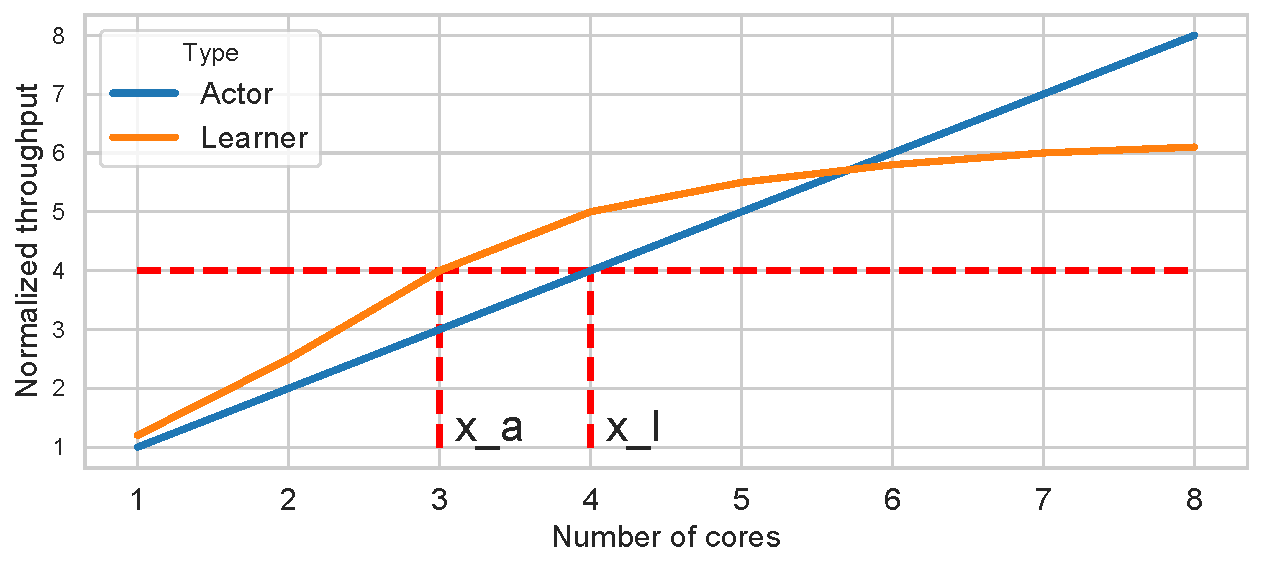
\includegraphics[width=\linewidth]{design_space.pdf}
    \caption{Illustration of design space exploration}
    \label{fig:design_space}
\end{figure}

As discussed in Section~\ref{sec:design_space_exp}, the objective is to allocate the number of cores for actors and learners, respectively such that the desired throughput ratio of the data collection and the data consumption is met. Our framework will first profile the throughput curve of actors and learners. We show an example in Figure~\ref{fig:design_space}, where the desired throughput ratio is 1. Then, we perform exhaustive search to find the solution $x_a$ and $x_b$ of Equation~\ref{eq:design_space}. The time complexity of the exhaustive search is $O(M^2)$, where $M$ is the total number of cores in the processor.

\subsection{Impact of the Data Layout}
The total size of the sum tree used in a typical replay buffer of size 1 million is less 10 KB. This makes the whole sum tree fit into the L2 cache of the modern CPUs. Thus, we only observe around $1\%$ benefit of our proposed cache aligned data layout. However, as the increase of the replay buffer size on larger problems, the superiority of our proposed data layout will appear.
